\documentclass[11pt,letterpaper]{article}
\usepackage{xcolor}
\usepackage{textcomp,marvosym}
\usepackage{amsmath,amssymb}
\usepackage[left]{lineno}
\usepackage{changepage}
\usepackage{rotating}
\usepackage{natbib}
\usepackage{setspace}
\usepackage{fancyhdr}
\usepackage{graphicx}
\usepackage{sidecap}
\usepackage{pdfpages}
\usepackage{longtable}
\usepackage{url}
\usepackage[aboveskip=1pt,labelfont=bf,labelsep=period,justification=raggedright,singlelinecheck=off]{caption}
%\doublespacing

\raggedright
\textwidth = 6.5 in
\textheight = 8.5 in
\oddsidemargin = 0.0 in
\evensidemargin = 0.0 in
\topmargin = -0.5 in
\headheight = 0.0 in
\headsep = 0.5 in
\parskip = 0.0 in
\parindent = 0.2 in

\begin{document}
\renewcommand{\thefigure}{S\arabic{figure}}
\renewcommand{\thetable}{S\arabic{table}}
\subsection*{Supporting Information for ``Synchronous emplacement of the anorthosite xenolith-bearing Beaver River diabase and one of the largest lava flows on Earth"}
Yiming Zhang, Nicholas L. Swanson-Hysell, Mark D. Schmitz, James D. Miller Jr., Margaret S. Avery

\subsection*{Bias Corrected Estimation of Paleointensity}
While using a set of selection criteria for excluding specimens with non-ideal paleointensity results is one common way of performing data analyses, the selection criteria themselves are often user-determined according to interpretations of certain groups of magnetic mineralogy on a case-by-case basis. The operation of performing a binary selection (accept or reject) on specimen results thus has an underlying assumption that the magnetic grain assemblage of specimens that pass the selection have a determined type of magnetic mineralogy. However, natural samples often have complex assemblage of magnetic carriers that span a range of composition, grain sizes and shapes. Thus, imposing a threshold value on certain parameters based on the paleointensity results can introduce bias from the analyzer. Alternatively, \citeA{Cych2021a} developed a Bias Corrected Estimation of Paleointensity (BiCEP) method that can eliminate biased introduced by using a set of arbitrarily defined selection criteria by taking all specimens into account for site-level paleointensity estimates. The method assumes that the paleointensity recorded by each specimen is biased away from a true value by an amount that is dependent on a single metric of nonlinearity (the curvature parameter $|\vec{k}|$; \citeA{Paterson2011a}) on the Arai plot. Although this method has the advantage of mitigating paleointensity estimate bias, it does not account for specimens that experience detrimental magnetic mineralogy alteration during heating steps unless such specimens are omitted before the analyses. 

We apply the BiCEP method to all sites in this study and the cooling rate corrected site-level paleointensity estimates are shown in Figure \ref{fig:BiCEP}. For the anorthosite sites (e.g. AX11) that show good specimen-level consistency (Figure \ref{fig:PINT_cooling_corrected}) and straight specimen Arai plots (Figure \ref{fig:IZZI_examples}), the paleointensity estimates derived from the BiCEP method using all specimen data is indistinguishable with that derived from the site average value based on selected specimens (Figure \ref{fig:PINT_cooling_corrected}). For anorthosites that show rather large specimen-level dispersion (e.g. AX8), or diabase sites that have double-slop behaviors and significant MD component, the paleointensity estimates using the BiCEP method tend to have broader uncertainty ranges and the median values are lower than those from anorthosites that typically have more ideal paleointensity behaviors (Figure \ref{fig:PINT_cooling_corrected}). Overall, site mean value of the mean probability distribution of the BiCEP method results is consistent with the weighted mean value of the selection criteria-based estimates. In addition, the majority of the anorthosite sites give high probability estimate for there being a geomagnetic field value \textit{ca.} 1092 Ma at a paleolatitude of $\sim$30\textdegree similar to that of today. This result is consistent with the interpretation that the anorthosite xenoliths record a high geomagnetic field during the late Mesoproterozoic.



\begin{figure}[h!]
\noindent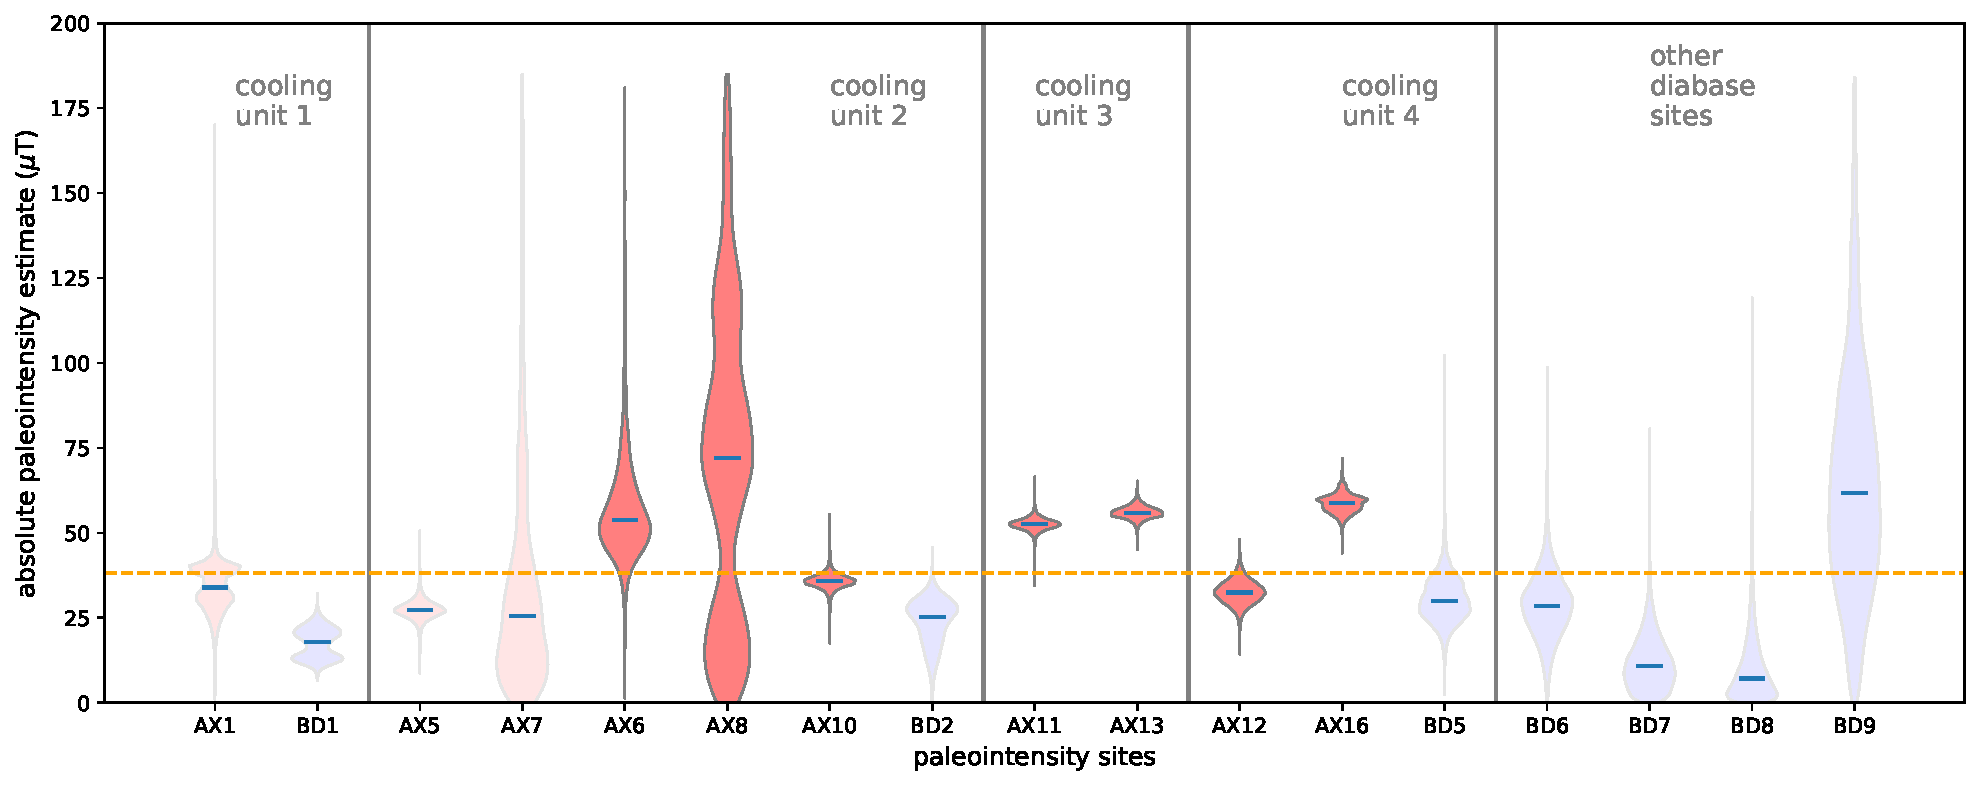
\includegraphics[width=\textwidth]{code/code_output/AX_BD_BiCEP.pdf}
\centering
\caption{\footnotesize{Violin plot of paleointensity estimates from the anorthosite and diabase using the bias corrected estimation of paleointensity (BiCEP) method \cite{Cych2021a}. The results are grouped by individual cooling units following \citeA{Zhang2021b}. All estimates are corrected for cooling rate by a factor of 0.74. }}
\label{fig:BiCEP}
\end{figure}



\clearpage


\bibliographystyle{gsabull}
\bibliography{YZ_ref}

\end{document}

